% WORKSHOP PAPER. 5 pages excluding references.
% Filename matches the Overleaf file so an upload overwrites it cleanly. Do not rename.
% The pristine template body is kept beside this as template_original.tex.
%
% Option 6, workshop with double-blind review. Verified in neurips_2026.sty:
% dblblindworkshop leaves \if@anonymous true, so the author block renders as
% "Anonymous Author(s)" automatically. sglblindworkshop would NOT.
%
% LAYOUT TARGET, from the professor, 24 August:
%   page 1        abstract + introduction
%   page 2 top    the method diagram. He called this extremely important.
%   page 2 rest   method
%   page 3 to 5 top   results, carrying all four tables
%   page 5 rest   conclusion and future work
%   after that    references, which do not count toward the five pages
% This draft is deliberately OVER length. He asked for everything in first, then
% he will help decide the cuts. Do not cut anything without asking.

\documentclass{article}

\usepackage[dblblindworkshop]{neurips_2026}

\usepackage[utf8]{inputenc}
\usepackage[T1]{fontenc}
\usepackage{hyperref}
\usepackage{url}
\usepackage{booktabs}
\usepackage{amsfonts}
\usepackage{nicefrac}
\usepackage{microtype}
\usepackage{xcolor}
\usepackage{graphicx}
\usepackage{tikz}
\usetikzlibrary{positioning,arrows.meta,fit,backgrounds}

% Every number lives in numbers.tex so this paper and long.tex cannot disagree.
% numbers.tex
%
% Every number either paper cites, defined once.
% Both neurips_2026.tex (workshop, 5 pages) and long.tex \input this file,
% so the two papers cannot drift apart.
%
% Rule: a macro is added here only after the figure exists in docs/paper_numbers.md
% with an n and a reproducing script. See that file's rule 1.
% The section number in each comment points into docs/paper_numbers.md.
%
% Naming: LaTeX control sequences cannot contain digits, so 3B is ThreeB
% and 7B is SevenB throughout.


% ---------------------------------------------------------------------------
% Splits and sample sizes
% ---------------------------------------------------------------------------

\newcommand{\nDev}{700}                  % testmini, development split
\newcommand{\nTest}{1{,}700}             % test.json, held-out split
\newcommand{\nIE}{600}
\newcommand{\nMATH}{600}
\newcommand{\nKNOW}{500}


% ---------------------------------------------------------------------------
% Headline accuracy, strict scoring, n = 1,700 held out. Section 2.18
% ---------------------------------------------------------------------------

\newcommand{\accThreeB}{59.8\%}
\newcommand{\accThreeBcount}{1016/1700}
\newcommand{\accThreeBci}{57.4--62.1}

\newcommand{\accSevenB}{67.8\%}
\newcommand{\accSevenBcount}{1153/1700}
\newcommand{\accSevenBci}{65.6--70.0}

\newcommand{\accRouted}{75.8\%}
\newcommand{\accRoutedcount}{1289/1700}
\newcommand{\accRoutedci}{73.7--77.8}

\newcommand{\accCloud}{77.4\%}
\newcommand{\accCloudcount}{1315/1700}
\newcommand{\accCloudci}{75.3--79.3}

\newcommand{\gainOverSevenB}{8.0}        % routed minus 7B alone
\newcommand{\gainOverThreeB}{16.0}       % routed minus 3B alone


% ---------------------------------------------------------------------------
% Routed against cloud alone, paired McNemar on identical claims. Section 2.18
% ---------------------------------------------------------------------------

\newcommand{\mcnemarAllP}{0.119}
\newcommand{\mcnemarAllDisagree}{258}
\newcommand{\mcnemarAllRoutedWins}{116}
\newcommand{\mcnemarAllCloudWins}{142}

\newcommand{\mcnemarIEP}{0.007}          % the one significant result, routed loses
\newcommand{\mcnemarIEDisagree}{109}
\newcommand{\mcnemarMATHP}{1.000}
\newcommand{\mcnemarKNOWP}{0.917}


% ---------------------------------------------------------------------------
% Per subset, all four arms. Section 2.18
% ---------------------------------------------------------------------------

\newcommand{\accThreeBIE}{63.3\%}
\newcommand{\accThreeBMATH}{57.3\%}
\newcommand{\accThreeBKNOW}{58.4\%}

\newcommand{\accSevenBIE}{68.5\%}
\newcommand{\accSevenBMATH}{66.5\%}
\newcommand{\accSevenBKNOW}{68.6\%}

\newcommand{\accRoutedIE}{77.5\%}
\newcommand{\accRoutedMATH}{77.3\%}
\newcommand{\accRoutedKNOW}{72.0\%}

\newcommand{\accCloudIE}{82.3\%}
\newcommand{\accCloudMATH}{77.2\%}
\newcommand{\accCloudKNOW}{71.6\%}

\newcommand{\escRateIE}{36.5\%}
\newcommand{\escRateMATH}{79.8\%}
\newcommand{\escRateKNOW}{42.0\%}


% ---------------------------------------------------------------------------
% Contribution 2: same-family agreement is correlated error. Section 2.18
% The whole FDV-IE deficit sits on claims the gate kept local.
% ---------------------------------------------------------------------------

\newcommand{\keptLocalIEn}{381}
\newcommand{\keptLocalIERouted}{76.9\%}
\newcommand{\keptLocalIECloud}{85.6\%}
\newcommand{\keptLocalIEGap}{8.7}        % points, routed below cloud

\newcommand{\escalatedIEn}{219}
\newcommand{\escalatedIERouted}{78.5\%}
\newcommand{\escalatedIECloud}{76.7\%}   % routed is slightly ahead here


% ---------------------------------------------------------------------------
% Escalation earns its cost. Section 2.18
% ---------------------------------------------------------------------------

\newcommand{\cloudCalls}{908}
\newcommand{\escWouldThreeB}{45.7\%}
\newcommand{\escWouldSevenB}{60.8\%}
\newcommand{\escCloudGave}{75.8\%}
\newcommand{\escGain}{15.0}              % points over the 7B on the same claims

\newcommand{\trigDisagreeN}{459}
\newcommand{\trigDisagreeSevenB}{57.3\%}
\newcommand{\trigDisagreeCloud}{73.4\%}
\newcommand{\trigDisagreeGain}{16.1}

\newcommand{\trigNumericN}{449}
\newcommand{\trigNumericSevenB}{64.4\%}
\newcommand{\trigNumericCloud}{78.2\%}
\newcommand{\trigNumericGain}{13.8}


% ---------------------------------------------------------------------------
% Routing behaviour. Section 2.18
% ---------------------------------------------------------------------------

\newcommand{\escalationRate}{53.4\%}     % claims that called the cloud
\newcommand{\onDeviceRate}{46.6\%}       % claims answered entirely on device
\newcommand{\localsAgreeRate}{66.2\%}
\newcommand{\accKeptLocal}{75.9\%}
\newcommand{\accCloudCalled}{75.8\%}


% ---------------------------------------------------------------------------
% Cost, from our own recorded token counts. Section 2.18, and 2.18.1 and 3.5
% USD and tokens only. Never CNY.
% ---------------------------------------------------------------------------

\newcommand{\costRouted}{\$1.066}
\newcommand{\costCloud}{\$1.882}
\newcommand{\costRatio}{56.6\%}
\newcommand{\tokensRoutedIn}{3{,}400{,}854}
\newcommand{\tokensRoutedOut}{2{,}106{,}383}
\newcommand{\tokensCloudIn}{6{,}319{,}626}
\newcommand{\tokensCloudOut}{3{,}560{,}933}
\newcommand{\medianLatency}{26.0}        % seconds per claim, GPU box, report median not mean


% ---------------------------------------------------------------------------
% Oracles. Upper bounds only. Neither may be presented as a system result.
% Section 2.18
% ---------------------------------------------------------------------------

\newcommand{\oracleThreeWay}{84.8\%}
\newcommand{\oracleThreeWayci}{83.0--86.4}
\newcommand{\oracleLocalOnly}{79.9\%}    % beats the cloud with zero cloud calls
\newcommand{\oracleLocalOnlyci}{78.0--81.8}


% ---------------------------------------------------------------------------
% Unparseable output. Section 2.18
% Cloud denominator is calls made, not 1,700.
% ---------------------------------------------------------------------------

\newcommand{\unparseThreeB}{1.65\%}
\newcommand{\unparseSevenB}{2.82\%}
\newcommand{\unparseCloud}{1.65\%}
\newcommand{\unparseRouted}{0.94\%}


% ---------------------------------------------------------------------------
% Retrieval, macro recall at k = 10. Section 1 and 2.16
% These are retrieval results. They may NOT be written as accuracy drivers.
% ---------------------------------------------------------------------------

\newcommand{\recallOursDev}{74.60\%}
\newcommand{\recallOursTest}{75.16\%}
\newcommand{\recallEmbedDev}{68.01\%}    % text-embedding-3-large, best published
\newcommand{\recallEmbedTest}{69.75\%}
\newcommand{\recallUpstreamBMDev}{65.16\%}
\newcommand{\recallUpstreamBMTest}{64.29\%}
\newcommand{\recallContrieverDev}{33.48\%}
\newcommand{\recallContrieverTest}{35.02\%}

\newcommand{\recallGainDev}{6.6}         % points over best published, testmini
\newcommand{\recallGainTest}{5.4}        % points over best published, held out

\newcommand{\recallElementTest}{70.0\%}
\newcommand{\recallAllGoldTest}{49.4\%}

\newcommand{\recallOursIETest}{77.92\%}
\newcommand{\recallOursMATHTest}{80.92\%}
\newcommand{\recallOursKNOWTest}{64.94\%}

% Why ours beats upstream's BM25: an implementation gap, priced.
\newcommand{\ablationIDF}{2.51}          % Lucene IDF, points
\newcommand{\ablationPunct}{2.02}        % dropping punctuation tokens, points
\newcommand{\ablationStem}{0.06}         % stemming, worth nothing
\newcommand{\tableInflation}{1.81}       % punctuation inflates table length this much
\newcommand{\paraInflation}{1.13}        % against this for paragraphs

% Fusion is dead on both splits.
\newcommand{\recallFusionTest}{74.95\%}  % below our BM25 alone


% ---------------------------------------------------------------------------
% Contribution 4: the error taxonomy. Section 2.17
% ---------------------------------------------------------------------------

\newcommand{\missingInfoKnowDev}{63.5\%}
\newcommand{\missingInfoKnowTest}{63.4\%}
\newcommand{\missingInfoAllTest}{41.0\%}
\newcommand{\missingInfoCiteRateTest}{38.4\%}
\newcommand{\missingInfoWrongTest}{47.6\%}
\newcommand{\missingInfoBaseTest}{35.8\%}


% ---------------------------------------------------------------------------
% The refuted bias, replicated four times. Section 2.18
% Share of claims each arm answers "entailed", where gold is 50.1% entailed.
% ---------------------------------------------------------------------------

\newcommand{\saysEntailedThreeB}{39.5\%}
\newcommand{\saysEntailedSevenB}{49.2\%}  % the only nearly calibrated arm
\newcommand{\saysEntailedRouted}{41.1\%}
\newcommand{\saysEntailedCloud}{33.9\%}
\newcommand{\saysEntailedGold}{50.1\%}

\newcommand{\entailedRouted}{67.1\%}
\newcommand{\entailedCloud}{61.7\%}
\newcommand{\refutedRouted}{84.6\%}
\newcommand{\refutedCloud}{93.1\%}


% ---------------------------------------------------------------------------
% The target device. Hard constraint, not a result. CLAUDE.md and section 3.1
% ---------------------------------------------------------------------------

\newcommand{\deviceLatency}{7}           % minutes per example, 3B on the MacBook
\newcommand{\deviceSecPerToken}{0.0641}
\newcommand{\deviceRsq}{0.995}
\newcommand{\deviceMeanPrompt}{6{,}610}  % tokens


% TITLE IS A PLACEHOLDER AND NEEDS YOUR APPROVAL.
\title{Routing Financial Claim Verification Between On-Device and Cloud Models}

% Fills the first-page footnote: "... (NeurIPS 2026). Workshop: <this>."
% Was unset since 10 August.
\workshoptitle{On-Device Intelligence: Foundation Models under Real-World Constraints}

% Double-blind. The style file replaces this block with "Anonymous Author(s)",
% so nothing here reaches the PDF. It is filled in for the camera-ready only.
\author{%
  Anonymous Author(s) \\
  Affiliation \\
  Address \\
  \texttt{email} \\
}

\begin{document}

\maketitle

\begin{abstract}
Financial claim verification often requires grounding short claims in long regulatory filings, making cloud-only inference costly and potentially unsuitable for sensitive documents. We build a routed edge--cloud pipeline that runs two small models on device and escalates only when a disagreement gate or an arithmetic trigger fires, with no training or fine-tuning. On \nTest{} held-out claims from FINDVER, the routed system reaches \accRouted{} accuracy versus \accCloud{} for a cloud-only baseline, with no significant overall difference, while using \costRatio{} of the cloud tokens and settling \onDeviceRate{} of claims entirely on device. The aggregate tie, however, hides a significant loss on one subset: agreement between two models of the same family becomes false confidence because their errors are correlated, costing \keptLocalIEGap{} points on information-extraction claims. Arithmetic claims show the complementary failure mode, where both local models fail in the same direction and an unconditional trigger succeeds where disagreement cannot. These results show that effective edge--cloud verification depends not only on local model accuracy, but on whether the routing signal can observe the failures that matter.

\end{abstract}

\section{Introduction}
\label{sec:intro}
Financial claim verification often requires grounding short claims in long, heterogeneous regulatory filings, documents that run to hundreds of pages \citep{reddy2024docfinqa}. Accuracy remains low even for frontier systems: given a retrieval system over such filings, GPT-4-Turbo answered 81\% of a manually reviewed sample of questions incorrectly or refused to answer \citep{islam2023financebench}. Sending every filing to a frontier cloud model is a poor deployment fit: filings may be commercially sensitive, while most input tokens come from the document rather than the claim, making repeated verification costly. Local models reduce both exposure and cost, but deciding when to trust them is difficult. The usual test is agreement: two local models read the same claim, and only a disagreement between them sends it to the cloud. That test assumes the two models fail independently, and some systematic failures produce no disagreement at all.

We address this problem with a routed edge--cloud verification pipeline that requires no training or fine-tuning. Retrieval and local inference remain on device, while a gate escalates only selected claims to a frontier model. We evaluate this design on FINDVER \citep{zhao2024findver}, where each claim must be judged \emph{entailed} or \emph{refuted} against the SEC filing it refers to. The strongest published system on that benchmark reaches \pubBestRAG{} under retrieval augmentation, and human experts reach \pubHumanExpert{}.

This paper makes three contributions. We measure what a routed pipeline gives up against a frontier cloud model, and find no significant difference at \escRate{} of the cloud calls. We show that the aggregate result is misleading, because a gate built on agreement between two models of one family reads correlated error \citep{kim2025correlated} as confidence, and we quantify what that costs on the subset where it happens. We then address the two failures the gate cannot see, agreement on a wrong verdict and arithmetic error the two models share, on the device.




% Claims about a company's financial performance circulate faster than the documents that
% would settle them, and settling one means reading a filing that runs to tens of thousands of
% words. FINDVER \citep{zhao2024findver} formalises the task: given a claim and the SEC filing
% it refers to, a system must decide whether the filing entails or refutes the claim. The
% filings average roughly 41,000 words and interleave narrative text with dozens of tables.
% The strongest published system, a frontier cloud model, reaches 77.2\% on them, whereas
% human financial experts reach 93.3\%.

% The obvious approach, sending every filing to a frontier model, fits this setting badly.
% Filings under analysis are commercially sensitive before they are public, and a prompt on
% this task is dominated by retrieved document text and not by the claim, so the per-token
% price is paid on the document over and over. Whether a large model can verify a financial
% claim is already settled, so the deployment question is how little of that model a working
% system actually needs.

% \paragraph{Goal.}
% Our aim is to measure that quantity, not to argue for an architecture. We build a
% verification pipeline whose default path runs entirely on the user's own hardware and which
% consults a frontier cloud model only when a gate decides the local models should not be
% trusted. Nothing is trained or fine-tuned. We then put two questions to the system. How
% much accuracy does routing give up against sending everything to the cloud? And does the
% aggregate answer to that question survive being broken apart?

% To answer them in order: the routed pipeline ties the cloud-only baseline overall, and that
% aggregate does not survive being broken apart. The second answer is the more informative of
% the two. The tie is one significant loss and two ties, and the loss has a single
% identifiable cause, which lies in how we built the gate and not in the benchmark.

% \paragraph{Contributions.}
% \begin{enumerate}
% \itemsep0pt
% \item A routed edge-cloud pipeline that ties a frontier cloud model on \nTest{} held-out
% claims at \costRatio{} of the cloud cost, with \onDeviceRate{} of claims answered without
% the document leaving the device, and with no training at any stage
% (Section~\ref{sec:headline}).
% \item Evidence that correlated error \citep{kim2025correlated} is severe enough between two
% models of one family to break a deployment gate that treats their agreement as confidence.
% On the information-extraction subset that agreement costs \keptLocalIEGap{} points against a
% model that would have answered those claims correctly (Section~\ref{sec:ie}).
% \item A trigger that escalates arithmetic claims unconditionally. It beats a disagreement
% gate on precisely the claims such a gate cannot see, because both local models fail them in
% the same direction (Section~\ref{sec:triggers}).
% \item An error taxonomy on the held-out split in which one failure mode, the model declaring
% the evidence absent and refuting on that basis, accounts for \missingInfoKnowTest{} of
% knowledge-subset errors and \missingInfoAllTest{} of all errors
% (Section~\ref{sec:taxonomy}).
% \item A retrieval result obtained with no model and no API call: a BM25 baseline reaching
% \recallOursTest{} macro recall on the held-out split, \recallGainTest{} points above the
% strongest retriever published on this benchmark (Section~\ref{sec:retrieval}). We keep it a
% retrieval result and claim nothing further, because recall and answer quality are close to
% decoupled in our pipeline.
% \end{enumerate}

% \paragraph{Fit to this workshop.}
% The system addresses efficient inference under real-world constraints. It is built for a
% machine that cannot hold a frontier model, and we treat its cost, its escalation rate and
% its latency as first-class results, not as an appendix. The analysis addresses benchmarks
% and evaluation for real-world deployment. An aggregate accuracy can hide a significant
% per-subset regression, and a confidence signal can mislead in a way that only a paired
% comparison exposes. Both are failures of measurement, not of modelling, and the
% single-number protocol this benchmark is normally reported under makes both invisible.


\section{Related Work}
\label{sec:related}

FINDVER \citep{zhao2024findver} verifies claims against long SEC filings and separates them into information extraction (FDV-IE), numerical reasoning (FDV-MATH), and domain-knowledge (FDV-KNOW) subsets; because these documents exceed consumer-model context limits, evaluation typically uses fixed retrieval augmentation \citep{lewis2020rag}. The only other method we found evaluated on FINDVER is MACE \citep{saha2026mace}, which decomposes verification into three roles but uses the same large model for all of them; its smallest reported configuration holds roughly 27B of parameters resident, where our two local models hold 10B between them. We instead study how different models should be assigned to different roles under consumer-device constraints. For numerical reasoning, Program of Thoughts \citep{chen2022pot}, PAL \citep{gao2022pal} and TART \citep{lu2025tart} delegate the arithmetic to code instead of performing it in-model \citep{wei2022cot}; Section~\ref{sec:triggers} shows why that fails at our model scale.

Small-to-large routing is commonly formulated as a cascade \citep{moslem2026routing}, including in edge-cloud systems \citep{li2025collaborative}, with deferral based on uncertainty \citep{kotte2026ucci} or model agreement \citep{kolawole2025agreement,soiffer2025semantic}. However, model errors are correlated \citep{kim2025correlated}, and even multiple frontier judges may provide few independent signals \citep{kohli2026judges}; Section~\ref{sec:ie} examines this issue in our two-model gate.

Financial claim verification has itself moved quickly since FINDVER appeared, in FinGround \citep{guo2026finground}, VeriFin \citep{hall2026verifin} and FinVerBench \citep{panda2026finverbench}. None of the three is evaluated on FINDVER, and none targets a device that cannot hold a frontier model, which is the constraint that shapes our design.


% ---------------------------------------------------------------------------
% THE METHOD DIAGRAM. Professor, 24 August: "extremely important", and it belongs
% at the top of page 2. [t] floats it to the top of whatever page it lands on, so
% if it comes out on the wrong page the fix is to move this block earlier or later
% in the source, not to change the placement specifier.
%
% 26 Aug: the hand-drawn TikZ version was replaced by model_diagram.png. The TikZ
% source is in git history at commit 50c68bb if it is ever needed again.
%
% 3 Sep: the diagram is regenerable again. The ten original icons were recovered by
% cropping them out of the old PNG and now live in paper/diagram_icons/, and
% test_scripts/build_model_diagram.py redraws the whole figure from them. The
% pre-3-Sep PNG is in git at commit 00bb76f.
%
% 4 Sep: the redrawn figure replaces the one that was in the Overleaf project. It adds
% the audit and the arbiter, which Section 3.2 describes and the old figure did not
% show, and colour is now consistent: on the arbiter and audit edges, green keeps the
% claim on the device and red sends it to the cloud. The old figure used green for the
% arithmetic escalation, which sends a claim to the cloud. The caption was rewritten
% with the figure, since the old one described neither component.
% ---------------------------------------------------------------------------
\begin{figure}[t]
\centering
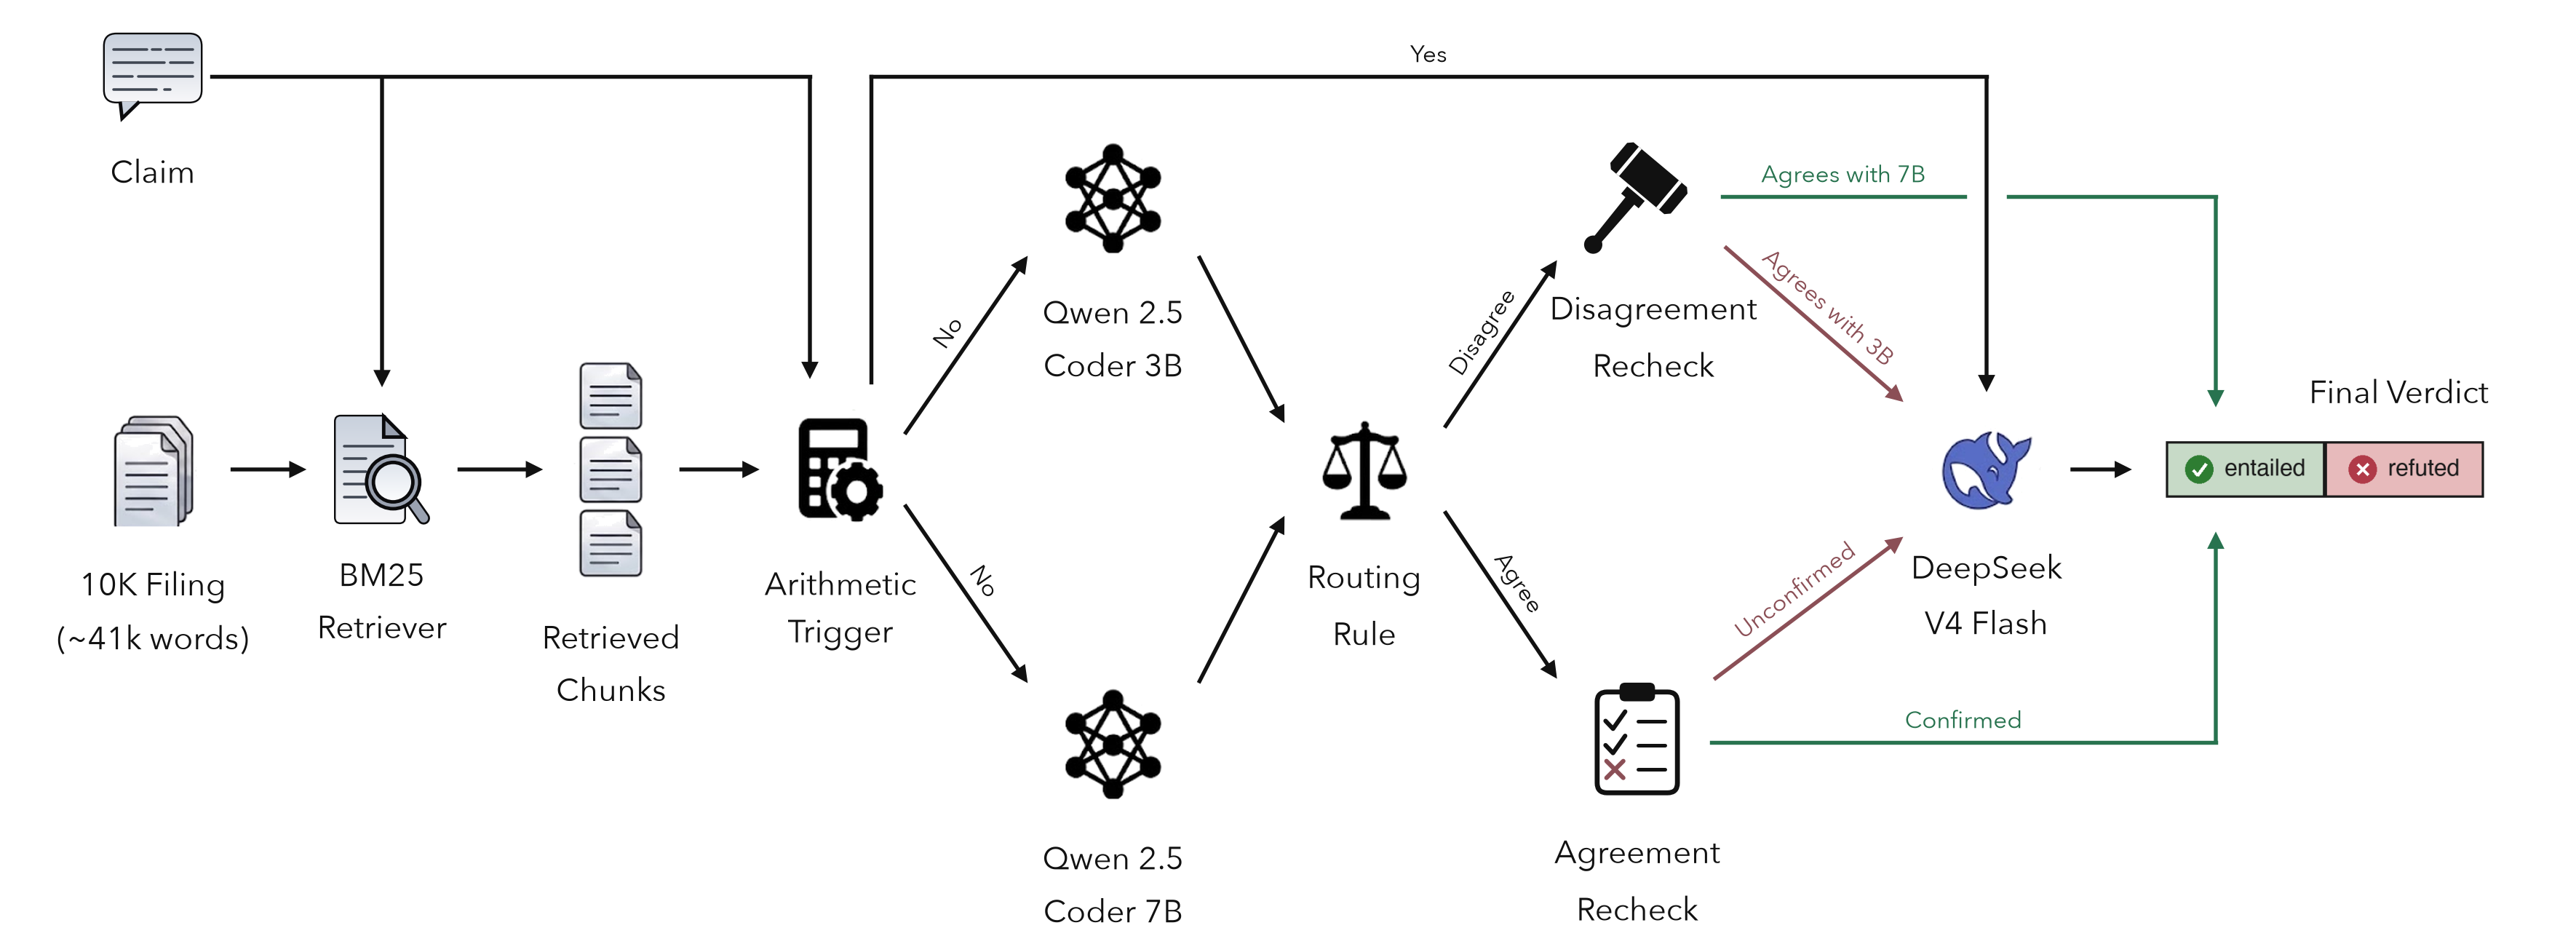
\includegraphics[width=\textwidth]{model_diagram.png}
\caption{The pipeline. Retrieval runs in plain Python with no model. Two small models on
the device read the same retrieved evidence and answer independently. The gate sends a
disagreement to the disagreement recheck and an agreement to the agreement recheck (Section~\ref{sec:routing}).
Green edges from those two components keep the claim on the device and red edges send it
to the cloud, which is reached on \fullEscRate{} of claims. A claim asserting a computed
quantity is escalated by the arithmetic trigger before either local model runs.}
\label{fig:pipeline}
\end{figure}




\section{Method}
\label{sec:method}

% \subsection{Pipeline}
% \label{sec:pipeline}
Given a claim and its regulatory filing, our system retrieves relevant evidence, attempts verification locally, and escalates only when the local tier is not trusted (Figure~\ref{fig:pipeline}). Retrieval and local inference run entirely on device; the cloud model is an exception path rather than the default. No component is trained or fine-tuned.

\subsection{On-Device Retrieval and Inference}
\label{sec:local}
We retrieve the top $k{=}10$ filing elements with BM25 \citep{robertson2009bm25}. The retriever uses no neural model or API call. The retrieved evidence is then given independently to Qwen2.5-Coder models with 3B and 7B parameters, both quantized to four bits and served through Ollama. They receive the same prompt and evidence, use a 32,768-token context window with temperature zero and a fixed seed, and do not observe each other's outputs.

The two models belong to the same family and were selected for deployment efficiency rather than diversity. This makes their agreement inexpensive to obtain but, as we show in Section~\ref{sec:ie}, not always a reliable confidence signal.

\subsection{Routing Policy}
\label{sec:routing}
Routing uses three signals. An arithmetic trigger, written in plain Python with no model behind it, handles arithmetic claims before local inference, and the gate escalates any claim on which the two local models disagree. We report those two together, without the rechecks, as \emph{gate only}. An agreement recheck then examines selected agreements and a disagreement recheck revisits disagreements, both on the device and each at the cost of at most one further 7B call. None of the three produces a verdict of its own; each only decides where the claim is answered. Whenever a claim is escalated, the cloud verdict replaces the local verdict.

\paragraph{Arithmetic Trigger.}
A fixed rule-based detector identifies claims that assert a computed quantity from the claim text alone. It uses three regular-expression patterns covering sentence-final numeric predicates, percentage claims, and approximate or exact numeric assertions. Detected claims are sent directly to the cloud. This trigger targets failures that disagreement cannot expose when both local models make the same arithmetic error.

\paragraph{Agreement Recheck.}
When both local models predict \emph{entailed}, we apply two checks for missed contradictions. First, a deterministic scan tests whether numerical values asserted by the claim occur anywhere in the filing under common formatting and scale variants. It is the only part of the system that reads outside the retrieved passages, and it runs no model and returns no verdict, so every verdict still comes from retrieved evidence alone. Second, the 7B model independently checks the retrieved evidence for an unsupported detail. Either signal triggers escalation; otherwise the shared local verdict is retained.

\paragraph{Disagreement Recheck.}
For non-arithmetic claims on which the local models disagree, the 7B model receives one additional query over the same evidence. Rather than asking it to choose between the previous verdicts, the prompt asks independently for evidence contradicting the claim. If the resulting verdict agrees with the 7B model's original answer, that answer is retained locally; otherwise the claim is escalated.

The two rechecks act on disjoint populations and each adds at most one additional local 7B call.


\section{Experimental Setup}
\label{sec:setup}
FINDVER provides no training data and our system has no trainable parameters, so its \nDev{}-claim development split is used only to select the retriever, $k$, local models, prompts and routing signals, and every figure is measured on the \nTest{}-claim test split. We report verdict accuracy under strict scoring, where a response with no recoverable verdict counts as incorrect, with the unparseable rate beside it. All latency measurements come from a consumer-GPU desktop; we do not report end-to-end latency on a CPU-only device, where the ordering of the local and cloud stages reverses. Appendix~\ref{appendix:setup} gives the scoring procedure, the configuration and the hardware in full.
\section{Results}
\label{sec:results}

\subsection{Routing matches cloud accuracy with fewer cloud calls}
\label{sec:headline}

\begin{table}[t]
\caption{Accuracy on \nTest{} held-out claims, strict scoring. The lower block is the
fraction of each subset that reached the cloud. Subsets are \nIE{}, \nMATH{} and \nKNOW{}
claims. Neither routed system differs significantly from the cloud-only baseline, at
$p = \mcnemarAllP{}$ for the gate alone and $p = \mcnemarFullP{}$ with both rechecks.}
\label{tab:accuracy}
\centering
\begin{tabular}{lcccc}
\toprule
system & overall & FDV-IE & FDV-MATH & FDV-KNOW \\
\midrule
3B alone                     & \accThreeB{}        & \accThreeBIE{}        & \accThreeBMATH{}        & \accThreeBKNOW{} \\
7B alone                     & \accSevenB{}        & \accSevenBIE{}        & \accSevenBMATH{}        & \accSevenBKNOW{} \\
routed, gate only            & \accRouted{}        & \accRoutedIE{}        & \accRoutedMATH{}        & \accRoutedKNOW{} \\
\textbf{routed, + both rechecks} & \textbf{\accFull{}} & \textbf{\accFullIE{}} & \textbf{\accFullMATH{}} & \textbf{\accFullKNOW{}} \\
cloud only                   & \accCloud{}         & \accCloudIE{}         & \accCloudMATH{}         & \accCloudKNOW{} \\
\midrule
escalated, gate only         & \escRate{}          & \escRateIE{}          & \escRateMATH{}          & \escRateKNOW{} \\
escalated, + both components & \fullEscRate{}      & \fullEscRateIE{}      & \fullEscRateMATH{}      & \fullEscRateKNOW{} \\
\bottomrule
\end{tabular}
\end{table}

Table~\ref{tab:accuracy} compares the routed system, with and without the two rechecks, against the cloud-only baseline. With the gate alone it reaches \accRouted{} accuracy against \accCloud{} for cloud-only inference. Their difference is not significant under paired McNemar testing ($p = \mcnemarAllP{}$), and that configuration was fixed before the test split was read.

Adding the two rechecks raises accuracy to \accFull{} ($p = \mcnemarFullP{}$) and reduces escalation from \escRate{} to \fullEscRate{}, leaving \fullOnDeviceRate{} of claims entirely on device and using \tokenRatioFull{} of the cloud input tokens of the cloud-only baseline (Table~\ref{tab:cost}). Both were designed after output from this split had been read, so we report them as a separate row (Appendix~\ref{sec:limitations}).

The cost reduction does not extend to latency. Both local models must run before most routing decisions can be made, so median end-to-end latency is \latRoutedMed{}\,s for the routed pipeline versus \latCloudMed{}\,s for cloud-only inference.

\begin{table}[t]
\caption{Cost and latency over the same \nTest{} held-out claims. Token counts are recorded
per claim. Latency is the GPU desktop; see Section~\ref{sec:setup}.}
\label{tab:cost}
\centering
\begin{tabular}{lccc}
\toprule
 & gate only & \textbf{full system} & cloud only \\
\midrule
cloud calls made              & \cloudCalls{}        & \textbf{\fullCloudCalls{}}   & \nTest{} \\
cloud input tokens            & \tokensRoutedIn{}    & \tokensFullIn{}    & \tokensCloudIn{} \\
cloud output tokens           & \tokensRoutedOut{}   & \tokensFullOut{}   & \tokensCloudOut{} \\
cloud cost                    & \costRouted{}        & \textbf{\costFull{}}        & \costCloud{} \\
claims answered on device     & \onDeviceRate{}      & \textbf{\fullOnDeviceRate{}} & 0\% \\
\midrule
median latency per claim      & \latRoutedMed{}\,s   & \latFullMed{}\,s   & \latCloudMed{}\,s \\
95th percentile latency       & \latRoutedPFive{}\,s & \latFullPFive{}\,s & \latCloudPFive{}\,s \\
\bottomrule
\end{tabular}
\end{table}

\subsection{Agreement can hide correlated error}
\label{sec:ie}

The aggregate result masks a failure of the basic disagreement gate. Table~\ref{tab:accuracy} shows that the gate-only system is significantly worse than the cloud baseline on FDV-IE, while the two systems are statistically tied on FDV-MATH and FDV-KNOW.

The deficit comes from claims the gate keeps locally. On the \keptLocalIEn{} FDV-IE claims retained on device, the routed system scores \keptLocalIERouted{}, whereas the cloud model would score \keptLocalIECloud{} on the same claims, a gap of \keptLocalIEGap{} points. By contrast, performance on escalated FDV-IE claims is comparable to the cloud baseline. The problem is therefore not insufficient escalation overall, but incorrect confidence in a particular set of agreements.

Because the two models share an architecture, a tokenizer and much of their training distribution, their errors are correlated: when both make the same mistake, agreement suppresses escalation exactly as if both were correct. Disagreement is therefore useful only to the extent that the models producing it fail differently.

The agreement recheck targets this failure mode. With the complete system, FDV-IE accuracy rises from \accRoutedIE{} to \accFullIE{}, and the difference from the cloud baseline is no longer significant ($p = \mcnemarFullIEP{}$). On locally retained FDV-IE claims, the gap to cloud performance narrows from \keptLocalIEGap{} to \fullKeptLocalIEGap{} points.

\subsection{The routing signals are complementary}
\label{sec:triggers}

\begin{table}[t]
\caption{The local and cloud verdicts on the claims each routing decision acts on.
\emph{Local} is the verdict the device would have returned and \emph{cloud} is the verdict
the cloud model returned or would have returned, scored on the same claims. The first three
rows are escalations. The fourth is a retention, where the disagreement recheck keeps the claim
on the device.}
\label{tab:routing}
\centering
\begin{tabular}{lccc}
\toprule
routing decision & claims & local & cloud \\
\midrule
escalate, the two models disagree& \trigDisagreeN{} & \trigDisagreeSevenB{}   & \trigDisagreeCloud{} \\
escalate, arithmetic claim       & \trigNumericN{}  & \trigNumericSevenB{}    & \trigNumericCloud{} \\
escalate, agreement recheck fires& \auditFired{}    & \auditLocalWouldScore{} & \auditCloudScored{} \\
keep, disagreement recheck sides with the 7B & \arbKept{}       & \arbKeptScore{}         & \arbCloudOnSame{} \\
\bottomrule
\end{tabular}
\end{table}

Over all \cloudCalls{} claims the gate escalated (Table~\ref{tab:routing}), the cloud model scores \escCloudGave{} against \escWouldSevenB{} for the 7B model had those claims been kept locally. The two original signals capture different errors: the arithmetic trigger operates on claims where the local models may agree, and therefore detects failures that disagreement cannot observe.

We also tested executing arithmetic locally rather than escalating it, following the Program-of-Thoughts pattern \citep{chen2022pot}. The approach failed at operand selection, not at execution: supplied with the correct operands the same deterministic interpreter reaches \arithOracle{}, but small local models often select the wrong figures from evidence containing many numerical candidates. Increasing the extractor from 3B to 7B narrows the gap to the cloud model without closing it, so we use arithmetic detection as a routing signal and not as a local solver.

Both rechecks separate the populations they examine. Of the \auditRan{} claims where the two local models agreed on \emph{entailed}, the agreement recheck passes claims that are correct \auditPassedScore{} of the time and flags the rest. The disagreement recheck keeps \arbKept{} of \arbRan{} non-arithmetic disagreements on the device at no cost in accuracy, and its signal is asymmetric: the 7B verdict is correct \arbSidedSevenBCorrect{} of the time when the recheck agrees with it, against \arbSidedThreeBCorrect{} when it does not.

\subsection{Missing evidence dominates the remaining errors}
\label{sec:taxonomy}

A single failure mode accounts for \missingInfoKnowTest{} of knowledge-subset errors and \missingInfoAllTest{} of all system errors, at a similar rate on the development split: the model states that the required evidence is absent and refutes the claim on that basis. The same pattern produces a broader label bias. Although \saysEntailedGold{} of gold labels are \emph{entailed}, the cloud model predicts that label on only \saysEntailedCloud{} of claims and the 3B model on only \saysEntailedThreeB{}, so failure to locate or interpret evidence is often converted into a refutation instead of an explicit abstention.

Finally, an oracle that selects the correct verdict whenever either local model produces it would reach \oracleLocalOnly{} without any cloud calls; allowing selection among both local models and the cloud model raises the bound to \oracleThreeWay{}. Neither is implementable, since each needs the gold label in order to select, but they show that a substantial fraction of the remaining error is attributable to routing and not to the absence of a correct candidate verdict.



\section{Conclusion}
\label{sec:conclusion}
% We studied how much frontier-model inference is actually necessary for financial claim verification under edge--cloud deployment constraints. A routed system can match cloud-only accuracy while keeping most verification local and substantially reducing cloud use, without training or fine-tuning. The main limitation is not simply local model accuracy, but the reliability of the signal used to decide when local predictions should be trusted.

% Our results show that disagreement is useful only for errors it can expose. Models from the same family can agree on the same mistake, turning correlated error into false confidence, while arithmetic failures can remain invisible when both local models fail in the same direction. Targeted routing signals recover some of these cases, but they also point to a broader design problem: an effective cascade must be built around the structure of its local errors, not agreement alone. More diverse local models and routing signals that detect shared failure modes are therefore promising directions for reducing cloud dependence further without hiding regressions behind aggregate accuracy.

We show that selective edge--cloud routing can match cloud-only accuracy on financial claim verification while substantially reducing cloud use. The main challenge is not local model accuracy alone, but whether the routing signal can detect shared failures: agreement between related models can become false confidence, and some errors remain invisible to disagreement. Effective cascades therefore need routing signals designed around the structure of local errors, not agreement alone.



\bibliographystyle{plainnat}
\bibliography{refs}

% \section*{NeurIPS Paper Checklist}

%%% BEGIN INSTRUCTIONS %%%
The checklist is designed to encourage best practices for responsible machine learning research, addressing issues of reproducibility, transparency, research ethics, and societal impact. Do not remove the checklist: {\bf The papers not including the checklist will be desk rejected.} The checklist should follow the references and follow the (optional) supplemental material.  The checklist does NOT count towards the page
limit. 

Please read the checklist guidelines carefully for information on how to answer these questions. For each question in the checklist:
\begin{itemize}
    \item You should answer \answerYes{}, \answerNo{}, or \answerNA{}.
    \item \answerNA{} means either that the question is Not Applicable for that particular paper or the relevant information is Not Available.
    \item Please provide a short (1--2 sentence) justification right after your answer (even for \answerNA). 
   % \item {\bf The papers not including the checklist will be desk rejected.}
\end{itemize}

{\bf The checklist answers are an integral part of your paper submission.} They are visible to the reviewers, area chairs, senior area chairs, and ethics reviewers. You will also be asked to include it (after eventual revisions) with the final version of your paper, and its final version will be published with the paper.

The reviewers of your paper will be asked to use the checklist as one of the factors in their evaluation. While \answerYes{} is generally preferable to \answerNo{}, it is perfectly acceptable to answer \answerNo{} provided a proper justification is given (e.g., error bars are not reported because it would be too computationally expensive'' or ``we were unable to find the license for the dataset we used''). In general, answering \answerNo{} or \answerNA{} is not grounds for rejection. While the questions are phrased in a binary way, we acknowledge that the true answer is often more nuanced, so please just use your best judgment and write a justification to elaborate. All supporting evidence can appear either in the main paper or the supplemental material, provided in appendix. If you answer \answerYes{} to a question, in the justification please point to the section(s) where related material for the question can be found.

IMPORTANT, please:
\begin{itemize}
    \item {\bf Delete this instruction block, but keep the section heading ``NeurIPS Paper Checklist"},
    \item  {\bf Keep the checklist subsection headings, questions/answers and guidelines below.}
    \item {\bf Do not modify the questions and only use the provided macros for your answers}.
\end{itemize} 
 

%%% END INSTRUCTIONS %%%


\begin{enumerate}

\item {\bf Claims}
    \item[] Question: Do the main claims made in the abstract and introduction accurately reflect the paper's contributions and scope?
    \item[] Answer: \answerTODO{} % Replace by \answerYes{}, \answerNo{}, or \answerNA{}.
    \item[] Justification: \justificationTODO{}
    \item[] Guidelines:
    \begin{itemize}
        \item The answer \answerNA{} means that the abstract and introduction do not include the claims made in the paper.
        \item The abstract and/or introduction should clearly state the claims made, including the contributions made in the paper and important assumptions and limitations. A \answerNo{} or \answerNA{} answer to this question will not be perceived well by the reviewers. 
        \item The claims made should match theoretical and experimental results, and reflect how much the results can be expected to generalize to other settings. 
        \item It is fine to include aspirational goals as motivation as long as it is clear that these goals are not attained by the paper. 
    \end{itemize}

\item {\bf Limitations}
    \item[] Question: Does the paper discuss the limitations of the work performed by the authors?
    \item[] Answer: \answerTODO{} % Replace by \answerYes{}, \answerNo{}, or \answerNA{}.
    \item[] Justification: \justificationTODO{}
    \item[] Guidelines:
    \begin{itemize}
        \item The answer \answerNA{} means that the paper has no limitation while the answer \answerNo{} means that the paper has limitations, but those are not discussed in the paper. 
        \item The authors are encouraged to create a separate ``Limitations'' section in their paper.
        \item The paper should point out any strong assumptions and how robust the results are to violations of these assumptions (e.g., independence assumptions, noiseless settings, model well-specification, asymptotic approximations only holding locally). The authors should reflect on how these assumptions might be violated in practice and what the implications would be.
        \item The authors should reflect on the scope of the claims made, e.g., if the approach was only tested on a few datasets or with a few runs. In general, empirical results often depend on implicit assumptions, which should be articulated.
        \item The authors should reflect on the factors that influence the performance of the approach. For example, a facial recognition algorithm may perform poorly when image resolution is low or images are taken in low lighting. Or a speech-to-text system might not be used reliably to provide closed captions for online lectures because it fails to handle technical jargon.
        \item The authors should discuss the computational efficiency of the proposed algorithms and how they scale with dataset size.
        \item If applicable, the authors should discuss possible limitations of their approach to address problems of privacy and fairness.
        \item While the authors might fear that complete honesty about limitations might be used by reviewers as grounds for rejection, a worse outcome might be that reviewers discover limitations that aren't acknowledged in the paper. The authors should use their best judgment and recognize that individual actions in favor of transparency play an important role in developing norms that preserve the integrity of the community. Reviewers will be specifically instructed to not penalize honesty concerning limitations.
    \end{itemize}

\item {\bf Theory assumptions and proofs}
    \item[] Question: For each theoretical result, does the paper provide the full set of assumptions and a complete (and correct) proof?
    \item[] Answer: \answerTODO{} % Replace by \answerYes{}, \answerNo{}, or \answerNA{}.
    \item[] Justification: \justificationTODO{}
    \item[] Guidelines:
    \begin{itemize}
        \item The answer \answerNA{} means that the paper does not include theoretical results. 
        \item All the theorems, formulas, and proofs in the paper should be numbered and cross-referenced.
        \item All assumptions should be clearly stated or referenced in the statement of any theorems.
        \item The proofs can either appear in the main paper or the supplemental material, but if they appear in the supplemental material, the authors are encouraged to provide a short proof sketch to provide intuition. 
        \item Inversely, any informal proof provided in the core of the paper should be complemented by formal proofs provided in appendix or supplemental material.
        \item Theorems and Lemmas that the proof relies upon should be properly referenced. 
    \end{itemize}

    \item {\bf Experimental result reproducibility}
    \item[] Question: Does the paper fully disclose all the information needed to reproduce the main experimental results of the paper to the extent that it affects the main claims and/or conclusions of the paper (regardless of whether the code and data are provided or not)?
    \item[] Answer: \answerTODO{} % Replace by \answerYes{}, \answerNo{}, or \answerNA{}.
    \item[] Justification: \justificationTODO{}
    \item[] Guidelines:
    \begin{itemize}
        \item The answer \answerNA{} means that the paper does not include experiments.
        \item If the paper includes experiments, a \answerNo{} answer to this question will not be perceived well by the reviewers: Making the paper reproducible is important, regardless of whether the code and data are provided or not.
        \item If the contribution is a dataset and\slash or model, the authors should describe the steps taken to make their results reproducible or verifiable. 
        \item Depending on the contribution, reproducibility can be accomplished in various ways. For example, if the contribution is a novel architecture, describing the architecture fully might suffice, or if the contribution is a specific model and empirical evaluation, it may be necessary to either make it possible for others to replicate the model with the same dataset, or provide access to the model. In general. releasing code and data is often one good way to accomplish this, but reproducibility can also be provided via detailed instructions for how to replicate the results, access to a hosted model (e.g., in the case of a large language model), releasing of a model checkpoint, or other means that are appropriate to the research performed.
        \item While NeurIPS does not require releasing code, the conference does require all submissions to provide some reasonable avenue for reproducibility, which may depend on the nature of the contribution. For example
        \begin{enumerate}
            \item If the contribution is primarily a new algorithm, the paper should make it clear how to reproduce that algorithm.
            \item If the contribution is primarily a new model architecture, the paper should describe the architecture clearly and fully.
            \item If the contribution is a new model (e.g., a large language model), then there should either be a way to access this model for reproducing the results or a way to reproduce the model (e.g., with an open-source dataset or instructions for how to construct the dataset).
            \item We recognize that reproducibility may be tricky in some cases, in which case authors are welcome to describe the particular way they provide for reproducibility. In the case of closed-source models, it may be that access to the model is limited in some way (e.g., to registered users), but it should be possible for other researchers to have some path to reproducing or verifying the results.
        \end{enumerate}
    \end{itemize}


\item {\bf Open access to data and code}
    \item[] Question: Does the paper provide open access to the data and code, with sufficient instructions to faithfully reproduce the main experimental results, as described in supplemental material?
    \item[] Answer: \answerTODO{} % Replace by \answerYes{}, \answerNo{}, or \answerNA{}.
    \item[] Justification: \justificationTODO{}
    \item[] Guidelines:
    \begin{itemize}
        \item The answer \answerNA{} means that paper does not include experiments requiring code.
        \item Please see the NeurIPS code and data submission guidelines (\url{https://neurips.cc/public/guides/CodeSubmissionPolicy}) for more details.
        \item While we encourage the release of code and data, we understand that this might not be possible, so \answerNo{} is an acceptable answer. Papers cannot be rejected simply for not including code, unless this is central to the contribution (e.g., for a new open-source benchmark).
        \item The instructions should contain the exact command and environment needed to run to reproduce the results. See the NeurIPS code and data submission guidelines (\url{https://neurips.cc/public/guides/CodeSubmissionPolicy}) for more details.
        \item The authors should provide instructions on data access and preparation, including how to access the raw data, preprocessed data, intermediate data, and generated data, etc.
        \item The authors should provide scripts to reproduce all experimental results for the new proposed method and baselines. If only a subset of experiments are reproducible, they should state which ones are omitted from the script and why.
        \item At submission time, to preserve anonymity, the authors should release anonymized versions (if applicable).
        \item Providing as much information as possible in supplemental material (appended to the paper) is recommended, but including URLs to data and code is permitted.
    \end{itemize}


\item {\bf Experimental setting/details}
    \item[] Question: Does the paper specify all the training and test details (e.g., data splits, hyperparameters, how they were chosen, type of optimizer) necessary to understand the results?
    \item[] Answer: \answerTODO{} % Replace by \answerYes{}, \answerNo{}, or \answerNA{}.
    \item[] Justification: \justificationTODO{}
    \item[] Guidelines:
    \begin{itemize}
        \item The answer \answerNA{} means that the paper does not include experiments.
        \item The experimental setting should be presented in the core of the paper to a level of detail that is necessary to appreciate the results and make sense of them.
        \item The full details can be provided either with the code, in appendix, or as supplemental material.
    \end{itemize}

\item {\bf Experiment statistical significance}
    \item[] Question: Does the paper report error bars suitably and correctly defined or other appropriate information about the statistical significance of the experiments?
    \item[] Answer: \answerTODO{} % Replace by \answerYes{}, \answerNo{}, or \answerNA{}.
    \item[] Justification: \justificationTODO{}
    \item[] Guidelines:
    \begin{itemize}
        \item The answer \answerNA{} means that the paper does not include experiments.
        \item The authors should answer \answerYes{} if the results are accompanied by error bars, confidence intervals, or statistical significance tests, at least for the experiments that support the main claims of the paper.
        \item The factors of variability that the error bars are capturing should be clearly stated (for example, train/test split, initialization, random drawing of some parameter, or overall run with given experimental conditions).
        \item The method for calculating the error bars should be explained (closed form formula, call to a library function, bootstrap, etc.)
        \item The assumptions made should be given (e.g., Normally distributed errors).
        \item It should be clear whether the error bar is the standard deviation or the standard error of the mean.
        \item It is OK to report 1-sigma error bars, but one should state it. The authors should preferably report a 2-sigma error bar than state that they have a 96\% CI, if the hypothesis of Normality of errors is not verified.
        \item For asymmetric distributions, the authors should be careful not to show in tables or figures symmetric error bars that would yield results that are out of range (e.g., negative error rates).
        \item If error bars are reported in tables or plots, the authors should explain in the text how they were calculated and reference the corresponding figures or tables in the text.
    \end{itemize}

\item {\bf Experiments compute resources}
    \item[] Question: For each experiment, does the paper provide sufficient information on the computer resources (type of compute workers, memory, time of execution) needed to reproduce the experiments?
    \item[] Answer: \answerTODO{} % Replace by \answerYes{}, \answerNo{}, or \answerNA{}.
    \item[] Justification: \justificationTODO{}
    \item[] Guidelines:
    \begin{itemize}
        \item The answer \answerNA{} means that the paper does not include experiments.
        \item The paper should indicate the type of compute workers CPU or GPU, internal cluster, or cloud provider, including relevant memory and storage.
        \item The paper should provide the amount of compute required for each of the individual experimental runs as well as estimate the total compute. 
        \item The paper should disclose whether the full research project required more compute than the experiments reported in the paper (e.g., preliminary or failed experiments that didn't make it into the paper). 
    \end{itemize}
    
\item {\bf Code of ethics}
    \item[] Question: Does the research conducted in the paper conform, in every respect, with the NeurIPS Code of Ethics \url{https://neurips.cc/public/EthicsGuidelines}?
    \item[] Answer: \answerTODO{} % Replace by \answerYes{}, \answerNo{}, or \answerNA{}.
    \item[] Justification: \justificationTODO{}
    \item[] Guidelines:
    \begin{itemize}
        \item The answer \answerNA{} means that the authors have not reviewed the NeurIPS Code of Ethics.
        \item If the authors answer \answerNo, they should explain the special circumstances that require a deviation from the Code of Ethics.
        \item The authors should make sure to preserve anonymity (e.g., if there is a special consideration due to laws or regulations in their jurisdiction).
    \end{itemize}


\item {\bf Broader impacts}
    \item[] Question: Does the paper discuss both potential positive societal impacts and negative societal impacts of the work performed?
    \item[] Answer: \answerTODO{} % Replace by \answerYes{}, \answerNo{}, or \answerNA{}.
    \item[] Justification: \justificationTODO{}
    \item[] Guidelines:
    \begin{itemize}
        \item The answer \answerNA{} means that there is no societal impact of the work performed.
        \item If the authors answer \answerNA{} or \answerNo, they should explain why their work has no societal impact or why the paper does not address societal impact.
        \item Examples of negative societal impacts include potential malicious or unintended uses (e.g., disinformation, generating fake profiles, surveillance), fairness considerations (e.g., deployment of technologies that could make decisions that unfairly impact specific groups), privacy considerations, and security considerations.
        \item The conference expects that many papers will be foundational research and not tied to particular applications, let alone deployments. However, if there is a direct path to any negative applications, the authors should point it out. For example, it is legitimate to point out that an improvement in the quality of generative models could be used to generate Deepfakes for disinformation. On the other hand, it is not needed to point out that a generic algorithm for optimizing neural networks could enable people to train models that generate Deepfakes faster.
        \item The authors should consider possible harms that could arise when the technology is being used as intended and functioning correctly, harms that could arise when the technology is being used as intended but gives incorrect results, and harms following from (intentional or unintentional) misuse of the technology.
        \item If there are negative societal impacts, the authors could also discuss possible mitigation strategies (e.g., gated release of models, providing defenses in addition to attacks, mechanisms for monitoring misuse, mechanisms to monitor how a system learns from feedback over time, improving the efficiency and accessibility of ML).
    \end{itemize}
    
\item {\bf Safeguards}
    \item[] Question: Does the paper describe safeguards that have been put in place for responsible release of data or models that have a high risk for misuse (e.g., pre-trained language models, image generators, or scraped datasets)?
    \item[] Answer: \answerTODO{} % Replace by \answerYes{}, \answerNo{}, or \answerNA{}.
    \item[] Justification: \justificationTODO{}
    \item[] Guidelines:
    \begin{itemize}
        \item The answer \answerNA{} means that the paper poses no such risks.
        \item Released models that have a high risk for misuse or dual-use should be released with necessary safeguards to allow for controlled use of the model, for example by requiring that users adhere to usage guidelines or restrictions to access the model or implementing safety filters. 
        \item Datasets that have been scraped from the Internet could pose safety risks. The authors should describe how they avoided releasing unsafe images.
        \item We recognize that providing effective safeguards is challenging, and many papers do not require this, but we encourage authors to take this into account and make a best faith effort.
    \end{itemize}

\item {\bf Licenses for existing assets}
    \item[] Question: Are the creators or original owners of assets (e.g., code, data, models), used in the paper, properly credited and are the license and terms of use explicitly mentioned and properly respected?
    \item[] Answer: \answerTODO{} % Replace by \answerYes{}, \answerNo{}, or \answerNA{}.
    \item[] Justification: \justificationTODO{}
    \item[] Guidelines:
    \begin{itemize}
        \item The answer \answerNA{} means that the paper does not use existing assets.
        \item The authors should cite the original paper that produced the code package or dataset.
        \item The authors should state which version of the asset is used and, if possible, include a URL.
        \item The name of the license (e.g., CC-BY 4.0) should be included for each asset.
        \item For scraped data from a particular source (e.g., website), the copyright and terms of service of that source should be provided.
        \item If assets are released, the license, copyright information, and terms of use in the package should be provided. For popular datasets, \url{paperswithcode.com/datasets} has curated licenses for some datasets. Their licensing guide can help determine the license of a dataset.
        \item For existing datasets that are re-packaged, both the original license and the license of the derived asset (if it has changed) should be provided.
        \item If this information is not available online, the authors are encouraged to reach out to the asset's creators.
    \end{itemize}

\item {\bf New assets}
    \item[] Question: Are new assets introduced in the paper well documented and is the documentation provided alongside the assets?
    \item[] Answer: \answerTODO{} % Replace by \answerYes{}, \answerNo{}, or \answerNA{}.
    \item[] Justification: \justificationTODO{}
    \item[] Guidelines:
    \begin{itemize}
        \item The answer \answerNA{} means that the paper does not release new assets.
        \item Researchers should communicate the details of the dataset\slash code\slash model as part of their submissions via structured templates. This includes details about training, license, limitations, etc. 
        \item The paper should discuss whether and how consent was obtained from people whose asset is used.
        \item At submission time, remember to anonymize your assets (if applicable). You can either create an anonymized URL or include an anonymized zip file.
    \end{itemize}

\item {\bf Crowdsourcing and research with human subjects}
    \item[] Question: For crowdsourcing experiments and research with human subjects, does the paper include the full text of instructions given to participants and screenshots, if applicable, as well as details about compensation (if any)? 
    \item[] Answer: \answerTODO{} % Replace by \answerYes{}, \answerNo{}, or \answerNA{}.
    \item[] Justification: \justificationTODO{}
    \item[] Guidelines:
    \begin{itemize}
        \item The answer \answerNA{} means that the paper does not involve crowdsourcing nor research with human subjects.
        \item Including this information in the supplemental material is fine, but if the main contribution of the paper involves human subjects, then as much detail as possible should be included in the main paper. 
        \item According to the NeurIPS Code of Ethics, workers involved in data collection, curation, or other labor should be paid at least the minimum wage in the country of the data collector. 
    \end{itemize}

\item {\bf Institutional review board (IRB) approvals or equivalent for research with human subjects}
    \item[] Question: Does the paper describe potential risks incurred by study participants, whether such risks were disclosed to the subjects, and whether Institutional Review Board (IRB) approvals (or an equivalent approval/review based on the requirements of your country or institution) were obtained?
    \item[] Answer: \answerTODO{} % Replace by \answerYes{}, \answerNo{}, or \answerNA{}.
    \item[] Justification: \justificationTODO{}
    \item[] Guidelines:
    \begin{itemize}
        \item The answer \answerNA{} means that the paper does not involve crowdsourcing nor research with human subjects.
        \item Depending on the country in which research is conducted, IRB approval (or equivalent) may be required for any human subjects research. If you obtained IRB approval, you should clearly state this in the paper. 
        \item We recognize that the procedures for this may vary significantly between institutions and locations, and we expect authors to adhere to the NeurIPS Code of Ethics and the guidelines for their institution. 
        \item For initial submissions, do not include any information that would break anonymity (if applicable), such as the institution conducting the review.
    \end{itemize}

\item {\bf Declaration of LLM usage}
    \item[] Question: Does the paper describe the usage of LLMs if it is an important, original, or non-standard component of the core methods in this research? Note that if the LLM is used only for writing, editing, or formatting purposes and does \emph{not} impact the core methodology, scientific rigor, or originality of the research, declaration is not required.
    %this research? 
    \item[] Answer: \answerTODO{} % Replace by \answerYes{}, \answerNo{}, or \answerNA{}.
    \item[] Justification: \justificationTODO{}
    \item[] Guidelines:
    \begin{itemize}
        \item The answer \answerNA{} means that the core method development in this research does not involve LLMs as any important, original, or non-standard components.
        \item Please refer to our LLM policy in the NeurIPS handbook for what should or should not be described.
    \end{itemize}

\end{enumerate}
% Commented out. checklist.tex is the NeurIPS main-conference questionnaire and the
% workshop probably does not require it. UNVERIFIED: check the workshop's call for papers
% before submitting. Template says checklist pages do not count toward the limit anyway.

\appendix

\section{Appendix}

\subsection{Limitations}
\label{sec:limitations}

\paragraph{Design and evaluation on the same split.}
The FDV-IE deficit and its mechanism were identified by reading the output of the held-out
run reported in Section~\ref{sec:ie}, and the two components of Section~\ref{sec:routing}
were designed in response to it and then evaluated on that same split. They therefore do not
carry the development-split protocol that the rest of the system follows, and we report them
as a separate system row in Table~\ref{tab:accuracy} rather than folding them into the
gate-only arm. The gate configuration reported there was frozen before that split was read
and is unaffected. Both components were also evaluated on the development split. The
cost reduction reproduces there almost exactly, from 54.0\% to 42.0\% of claims escalated
against 53.4\% to \fullEscRate{} here. Accuracy on that split is flat, 79.0\% with and
without the components, with FDV-IE at 83.6\% against 83.2\%; that split escalates a
comparable fraction of claims but its disagreement population is a harder one, and we report
the figure rather than resting the components' case on it.

\paragraph{One benchmark, one document type.}
Every result here comes from FINDVER, which is built on English-language SEC filings.
Neither the retriever's advantage nor the arithmetic trigger's precision should be assumed
to transfer to another document class, and the detector in particular exploits a
regularity of phrasing that may be an artefact of how these claims were written.

\paragraph{Reproducibility.}
The cloud endpoint does not honour a temperature or a seed, so its verdicts vary between
identical runs. Our own local models are seeded at temperature zero and still move roughly
one verdict in ten between reruns on the same machine. Comparisons in this paper are
therefore paired wherever a paired test is available.

\paragraph{No latency measurement on a CPU-only device.}
All timings come from the GPU desktop. The laptop that motivates the on-device framing has
been measured for a single local model only, and the routed pipeline has not been run on
it end to end.

\subsection{Detailed Experimental Settings}
\label{appendix:setup}
\paragraph{Splits and protocol.}
FINDVER provides a development split of \nDev{} claims and a test split of \nTest{} claims,
both with labels. The benchmark ships no training data, and no component of this system has
trained parameters, so development consists of selecting components and settings rather than
fitting them. We carry out that selection on the development split, including the retriever,
the value of $k$, the choice of local models, the prompts and both gate triggers, and we
report all figures on the test split. Reruns of an identical configuration on this hardware
move roughly one verdict in ten, so we treat any difference smaller than that as noise rather
than as a result.

\paragraph{Scoring.}
A verdict is extracted from the model's response by a rule-based extractor that searches the
whole response, not only its final sentence, since small models frequently place the verdict
elsewhere. Responses from which no verdict can be recovered are counted in an explicit
unparseable category and scored as incorrect, which we call strict scoring. We report the
unparseable rate alongside every accuracy figure, because a system that fails to answer and
a system that answers wrongly are different failures and strict scoring alone conflates
them. On the held-out split the rate is \unparseThreeB{} for the 3B model, \unparseSevenB{}
for the 7B, and \unparseRouted{} for the routed system. Where a figure of ours is placed
beside a published one, we additionally report it under the benchmark's own convention, in
which unrecoverable verdicts are resolved by a coin flip. Comparing a strictly scored number
with a coin-flipped one would understate ours by exactly the amount our models fail the
output format.

\paragraph{Hardware.}
Experiments were executed on a desktop with a consumer GPU, since a full run of the routed
pipeline over the test split takes about \latRunHours{} hours there. The device of record
for the deployment claim, however, is a 2017 laptop with 16\,GB of memory and no usable
GPU, and every latency figure must name its machine because the ordering reverses between
them. On the desktop the local 3B model is the fastest of the three at
\latThreeBMed{} seconds per claim, faster than either cloud model; on the laptop the same
model takes roughly 420 seconds. Every latency figure in this paper comes from the desktop.
We have not measured the routed pipeline end to end on the laptop.

\subsection{Retrieval}
\label{sec:retrievalresults}

Our BM25 retriever reaches \recallOursTest{} macro recall at $k{=}10$ on the held-out split, \recallGainTest{} points above the strongest retriever previously reported on FINDVER (Table~\ref{tab:recall}). The result uses no neural model and no API call.

The gain is largely an implementation effect rather than a new retrieval method. Development-set ablations attribute it mainly to the IDF formulation and punctuation handling; additional claim decomposition, dense fusion, and parameter sweeps do not improve the final retriever.

More importantly, retrieval recall is only weakly coupled to downstream verification in our pipeline. Supplying perfect evidence does not significantly improve accuracy ($p = 0.116$), while increasing $k$ from 10 to 20 substantially raises recall but produces no measurable accuracy gain despite increasing prompt length. We therefore report the BM25 result as a retrieval result, not as an explanation for the verification gains above.

\begin{table}[t]
\caption{Macro recall at $k{=}10$, the metric the benchmark's own evaluation script computes.
Our BM25 replicates to within 0.6 points on the held-out split it was never tuned on, and
beats the strongest published retriever there by \recallGainTest{} points with no neural
model and no API cost.}
\label{tab:recall}
\centering
\begin{tabular}{lcc}
\toprule
retriever & dev ($n{=}\nDev{}$) & held-out ($n{=}\nTest{}$) \\
\midrule
\textbf{ours, BM25}                & \textbf{\recallOursDev{}} & \textbf{\recallOursTest{}} \\
\texttt{text-embedding-3-large}    & \recallEmbedDev{}         & \recallEmbedTest{} \\
benchmark's BM25                   & \recallUpstreamBMDev{}    & \recallUpstreamBMTest{} \\
\texttt{contriever-msmarco}        & \recallContrieverDev{}    & \recallContrieverTest{} \\
\bottomrule
\end{tabular}
\end{table}

\subsection{Future Work}

A verification pipeline whose default path runs on consumer hardware ties a frontier cloud
model on \nTest{} held-out financial claims, at \costRatioFull{} of the cost, with
\fullOnDeviceRate{} of filings never leaving the device and with no training at any stage.
The aggregate tie has structure, and identifying that structure was what produced the two
components that close most of it.

The mechanism is specific and it is actionable. A gate built on agreement between two small
models reads correlated error as confidence, and because our two local models come from one
family their agreement on the information-extraction subset was worth
\keptLocalIEGap{} points on the claims the gate kept. The two components of
Section~\ref{sec:routing} address the two sides of that failure directly: the agreement recheck
re-examines the agreements the gate trusts, and the disagreement recheck resolves the ones it
does not. Together they narrow the FDV-IE deficit on kept claims from \keptLocalIEGap{} to
\fullKeptLocalIEGap{} points, raise overall accuracy from \accRouted{} to \accFull{}, and
remove \arbKept{} cloud calls, so that the system answers a majority of claims without
contacting the cloud at all. Both components are local, both cost at most one additional 7B
call, and neither requires a second model family or any training.

The general lesson is that the value of a cascade gate is bounded by the independence of the
signals it reads, and that when independence is unavailable it can be recovered cheaply by
asking the same model a different question. The disagreement recheck does not add a model; it adds a
question whose answer is informative precisely because it is not framed as a decision
between two known positions.

Three further directions come out of the measurements above. The escalation triggers are
hand-written, and the taxonomy in Section~\ref{sec:taxonomy} suggests a learned or
pattern-derived trigger aimed at the specific failure that dominates the error budget, which
the present gate does not detect at all. A trigger of that kind is one half of an agentic
skill in the sense now being formalised \citep{jiang2026skills}, a reusable procedure
carrying its own applicability condition; the other half, the procedure itself, is where the
interpreter we did not build would sit. The oracle bound indicates that most of the
remaining gap is a selection problem and not a capability problem, so a better gate is a
better investment than a better local model. Every latency figure here comes from a desktop,
so measuring the pipeline end to end on a CPU-only consumer machine is necessary before any claim
about deployability on that class of hardware, and we make none here.



\end{document}
